%%% Local Variables:
%%% TeX-command-extra-options: "-shell-escape"
%%% mode: latex
%%% TeX-master: t
%%% End:
\documentclass{beamer}
\usepackage{caption}
\usepackage{minted}
\usepackage{tikz}
\usepackage{xcolor}
\usetikzlibrary{shapes.geometric, arrows}
\tikzstyle{startstop} = [rectangle, rounded corners, minimum width=3cm, minimum height=1cm,text centered, draw=black, fill=red!30]
\tikzstyle{io} = [trapezium, trapezium left angle=70, trapezium right angle=110, minimum width=1.5cm, minimum height=0.6cm, text centered, draw=black, fill=blue!30]
\tikzstyle{process} = [rectangle, minimum width=1.5cm, minimum height=0.5cm, text centered, draw=black, fill=orange!30]
\tikzstyle{decision} = [circle, radius=2.5cm, text centered, draw=black, fill=green!30]
\tikzstyle{arrow} = [thick,->,>=stealth]
\usepackage[labelformat=simple]{subcaption}

\usetheme{Singapore}
\title{Arbitrarily Large Data}
\begin{document}
\begin{frame}
\titlepage
\end{frame}
\section{Lists}

\begin{frame}
  \huge \emph{Recursion} - see recursion
\end{frame}

\begin{frame}
  \frametitle{Self Referentiality Powerful and Scary}
  \begin{figure}
    \begin{subfigure}{0.3\textwidth}
      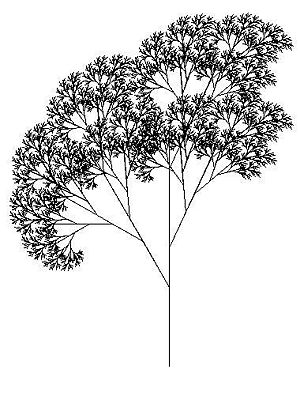
\includegraphics[width=0.9\textwidth]{images/recursive-tree.JPG}
    \end{subfigure}
    \begin{subfigure}{0.3\textwidth}
      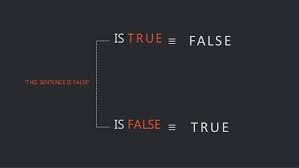
\includegraphics[width=0.9\textwidth]{images/liars-paradox.jpeg}
    \end{subfigure}
    \begin{subfigure}{0.3\textwidth}
      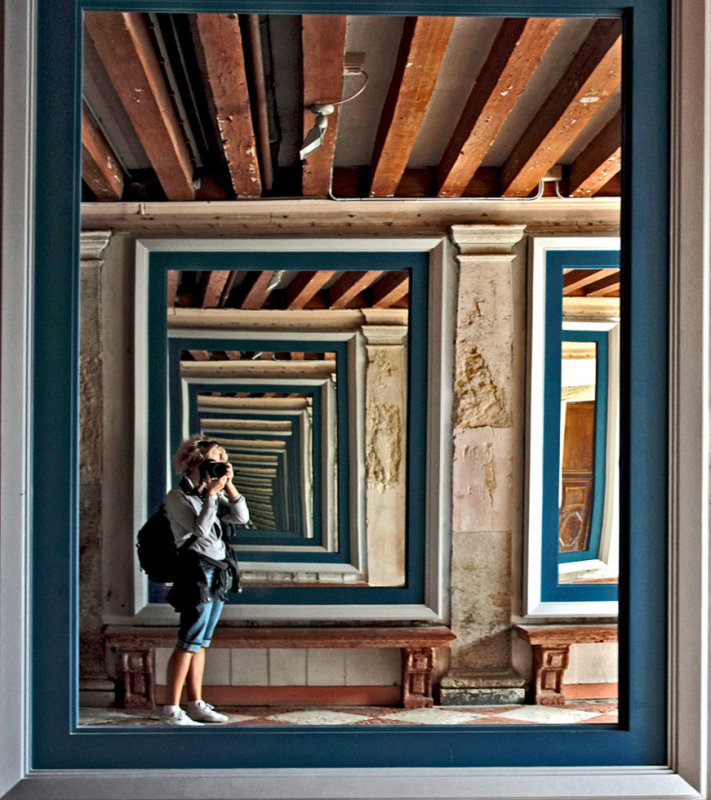
\includegraphics[width=0.9\textwidth]{images/reflections.jpg}
    \end{subfigure}
  \end{figure}
\end{frame}

\begin{frame}
  \frametitle{Self Referentiality}
  The ability to self reference is \emph{powerful} but also \emph{troublesome}.
  \begin{itemize}
  \item<2-> Through self referentiality, we can construct the most basic mathematical tool that has
    been proven to be a powerful concept throughout history--the natural numbers.
  \item<3-> This leads to many other powerful structures like other numbers, lists, trees, etc.
  \item<4-> But we also got the first instances of extremely troublesome concepts--paradoxes.
  \item<5-> The omnipotence paradox - asked if it was possible for a being to exist so powerful that it could create a stone that it could not lift.
  \item<6-> The Epimenides paradox, 'All Cretans are liars' when uttered by an ancient Greek Cretan was one of the first recorded versions. 
  \end{itemize}
\end{frame}

\begin{frame}
  \frametitle{Stacking Dolls and Us}
  \begin{center}
    \includegraphics[width=0.5\textwidth]{images/matryoshka.jpg}
  \end{center}
  Hello me, meet the previous me.\\
  -Dave Mustaine\\
  --Me
\end{frame}

\begin{frame}
  \frametitle{Self Referential Data and Racket}
  So far, we have only written programs with fixed size data (well numbers and strings aren't truly fixed size but they are primitive).
  \begin{itemize}
  \item<2-> We don't currently have a way to specify data definitions for extensible data.
  \item<3-> Consequently, we can't support the creation of programs like a space invaders game with
    flexible numbers of enemies.
  \item<4-> So we will change how we specify data definitions to support things like this and will revise our design recipes
    for dealing with extensible data
  \end{itemize}
\end{frame}

\begin{frame}
  \frametitle{Lists: A Fundamental Structure }
  One of the most important things to get used to in functional programming is dealing with lists.
  \begin{itemize}
  \item<2-> Lists are quite common in programming in general as a way to store related data for processing data.
  \item<3-> A large part of the execution time of many programs is spent iterating over lists.
  \item<4-> The simplest list we can specify is the empty list \mintinline{racket}{'()}
  \item<5-> We can start building lists with \mintinline{racket}{cons}--for example
    \mintinline{racket}{(cons 1 '())} $\hookrightarrow$ \mintinline{racket}{'(1)}.
  \item<6-> We can also use other types like strings in our lists \mintinline{racket}{(cons "Mercury" '())}
  \end{itemize}
\end{frame}

\begin{frame}
  \frametitle{Analyzing Cons Cells}
  Let's consider the following list: \mintinline{racket}{(cons "Mercury" '())}.
  \begin{itemize}
  \item<2-> We have the following visual representation of this list:
    \includegraphics[width=0.2\textwidth]{images/mercury-cons.png}
  \item<3-> For \mintinline{racket}{(cons "Earth" (cons "Venus" (cons "Mercury" '()))))}
    we have the following visual representation:
    \includegraphics[width=0.35\textwidth]{images/planet-cons.png}
  \end{itemize}
\end{frame}

\begin{frame}
  \frametitle{Cons Cell Properties}
  The nested representation of cons cells gets complicated as lists get larger, very quickly.
  \begin{itemize}
  \item<2-> Programmers usually opt to think about them in terms of box and pointer diagrams instead:
    \includegraphics[width=0.5\textwidth]{images/box-pointer-back.png}
  \item<3-> It's more natural to think about this in a more forward manner however, where the box on the
    left corresponds to the \emph{head} of the list and there is a pointer to the \emph{tail} of the list:
    \includegraphics[width=0.5\textwidth]{images/box-pointer-forward.png}
  \end{itemize}
\end{frame}

\begin{frame}
  \frametitle{Some Weird Lists}
  By this point, you may be used to thinking about lists as \emph{homogeneous} collections of items.
  \begin{itemize}
  \item<2-> But you can also creates lists from elements of different types:
    \mintinline{racket}{(cons "Peter" (cons 26 (cons \#t '())))}
  \item<3-> In this list we have a string, an integer, and a boolean value.
  \item<4-> We can also think about adding structs or functions to our list.
  \item<5-> Alternatively, instead of thinking about our list as being unstructured,
    we could say that is a list whose values are an itemization of strings, integers, and true.
  \item<6-> If we cons on a new value with a type not present in the itemization, then we could define
    an itemization that extends our previous one.
  \item<7-> And building on my previous lectures, we can even think of this list as representing
    something like a person. But in that case we should define a struct!
  \end{itemize}
\end{frame}

\defverbatim[colored]\ThreeList{
\begin{minted}[fontsize=\footnotesize]{racket}
    ; A 3LON is a list of three numbers: 
    ;   (cons Number (cons Number (cons Number '())))
    ; interpretation a point in 3-dimensional space 
\end{minted}
}

\begin{frame}
  \frametitle{Data Definitions and Lists}
  Consider the following list: \mintinline{racket}{(cons 1 (cons 2 (cons 3 '())))}
  \begin{itemize}
  \item<2-> What kind of data definition could we given for this list?
  \item<3-> \ThreeList
  \item<4-> Again, such a data definition seems more appropriate for struct.
  \item<5-> More importantly, the list is extensible and this definition
    doesn't address the fact that consing an additional element to
    the aforementioned list creates a value outside of this definition.
  \item<6-> So how do we talk about data definitions
    where we can construct values of arbitrarily large size?
  \end{itemize}
\end{frame}

\defverbatim[colored]\ListOfNames{
\begin{minted}[fontsize=\footnotesize]{racket}
    ; A List-of-names is one of: 
    ; – '()
    ; – (cons String List-of-names)
    ; interpretation a list of guests, by last name
\end{minted}
}

\begin{frame}
  \frametitle{Lists are Recursively Defined}
  Let's say that we are designing a program for hotel booking for a large
  hotel. For a given weekend we need a list of dynamic size for our
  guest list.
  \begin{itemize}
  \item<2-> Assuming we only store the guest's last name, how do we shape
    our data definition to meet this dynamic size requirement?
  \item<3-> \ListOfNames
  \item<4-> Such a definition should seem familiar to you at this point.
  \item<5-> When programming data structures in Java, you should have
    become used to recursive instances of a class in a class definition.
  \end{itemize}
\end{frame}

\begin{frame}
  \frametitle{List-of-names Examples}
  What are some example values of our List-of-names definition?
  \begin{itemize}
  \item<2-> Starting with the first clause of our definition's itemization,
    we have a nice atomic element.
  \item<3-> This element is the empty list \mintinline{racket}{'()} and forms the smallest  value in our list.
  \item<4-> The most simple elements of \emph{inductively} defined data are known
    as our base values, in correspondance with the \emph{base case} of an
    inductive proof.
  \item<5-> Don't worry about this too much for now, let's look
    at more values of our data definition.
  \item<6-> In order to construct a more complicated list, we look at the second clause of our itemization. We must cons a string
    onto another list, but so far we only know how to constuct the empty list.
  \item<7-> This allows us to define a single element list like:
    \mintinline{racket}{(cons "Nadal" '())}
  \end{itemize}
\end{frame}

\begin{frame}
  \frametitle{List-of-names Examples (cont.)}
  How do we create a two element guest list?
  \begin{itemize}
  \item<2-> Easy, we apply the second case of our itemization again and cons something onto a one element list!
  \item<3-> \mintinline{racket}{(cons "Federer" (cons "Nadal" '()))}
  \item<4-> And of course, we can inductively keep constructing an arbitrary
    list of size N+1 from a list of size N.
  \item<5-> This brings an interesting point up. Can I use induction to prove
    things about propositions that are generated from things besides natural numbers?
  \item<6-> Yes, inductively defined types come with their own induction principles. Programming language theorists do induction over different structures often.
  \item<7-> But back to programming land! We seemed to brush over some details.
    What exactly are \mintinline{racket}{'()} and \mintinline{racket}{cons}?
  \end{itemize}
\end{frame}

\section{Atoms and Constructors}
\begin{frame}
  \frametitle{Empty Lists and Cons}
  So, we've mentioned that \mintinline{racket}{'()} is a value, but what
  is special about it?
  \begin{itemize}
  \item<2-> Well, like numbers, booleans, and strings it is a new kind of \emph{atomic} value in our language.
    Struct values, the last new value form we introduced are compound values--i.e. they are composed
    of many other values.
  \item<3-> It is a unique value in that there is a built-in predicate to recognize it, \mintinline{racket}{empty?}
  \item<4-> \mintinline{racket}{(empty? '())} returns true and \mintinline{racket}{(empty? v)} returns false for any other
    value, v.
  \item<5-> And of course, we can start building lists containing elements by using \mintinline{racket}{cons} with it.
  \item<6-> So, what's the deal with \mintinline{racket}{cons}?
  \item<7-> Recall, when we defined a struct, how did we create new values for a struct type?
  \end{itemize}
\end{frame}

\begin{frame}
  \frametitle{Dissecting Cons}
  So, let's assume that we can define a struct for \mintinline{racket}{cons} as follows:
  \begin{itemize}
  \item<2-> \mintinline{racket}{(struct cons [first rest])}
  \item<3-> \mintinline{racket}{(cons 1 '())} seems to work as expected.
  \item<4-> We can also use a value that isn't a list as the ``rest'': \mintinline{racket}{(cons 1 2)}.
  \item<5-> For simplicity in the book, they don't allow this because they want you to think of cons cells as \emph{lists}.
  \item<6-> But in reality, a list is a series of cons pairs whose final ``rest'' is \mintinline{racket}{'()}.
  \item<7-> So, I recommend mostly using \mintinline{racket}{cons} for constructing lists, but you can also construct pairs.
  \item<8-> If you need to specify a larger list quickly, use
    something like \mintinline{racket}{'(1 2 3)} or \mintinline{racket}{(list 1 2 3)} instead of \mintinline{racket}{(cons 1 (cons 2 (cons 3 '())))}
  
  \end{itemize}
\end{frame}

\defverbatim[colored]\ContainsHeader{
\begin{minted}{racket}
    ; List-of-names -> Boolean
    ; determines whether "Smith" is in a-list-of-names
    (define (contains-smith? a-list-of-names)
      \#f)
\end{minted}
}

\begin{frame}
  \frametitle{List Programs}
  We can get the first element of a list with \mintinline{racket}{first} and the
  rest of the list with \mintinline{racket}{list}.
  \begin{itemize}
  \item<2-> With this, we can now start to write programs using lists.
  \item<3-> \textbf{Sample Problem} - You're the most popular person in town. You have lots of friends. So many in fact that you can't remember all of your friends' names. Assume that your friends are stored in a list. Write a program to check that you have a friend named ``Smith''.
  \item<4-> \ContainsHeader
  \item<5-> Ok, so now we need functional examples.
  \item<6-> What should \mintinline{racket}{(contains-smith? '())} return?
  \item<7-> It should return \#f of course!
  \end{itemize}
\end{frame}

\begin{frame}
  \frametitle{Recurring in the Lists}
  Ok, so we know that searching for Smith in the empty list returns false.
  \begin{itemize}
  \item<2-> What should \mintinline{racket}{(contains-smith? (cons "Trufant" '()))} return?
  \item<3-> It should return \#f since ``Trufant'' isn't ``Smith'' and
    the empty list doesn't contain any strings.
  \item<4-> What should \mintinline{racket}{(contains-smith? (cons "Smith" '()))} return?
  \item<5-> It should return \#t of course!
  \item<6-> What should \mintinline{racket}{(contains-smith? (cons "Junpei" (cons "Smith" '())))} return?
  \item<7-> Still \#t!
  \item<8-> What about \mintinline[fontsize=\footnotesize]{racket}{(contains-smith? (cons "Junpei" (cons "Smith" (cons "Trufant" '()))))}?
  \end{itemize}
\end{frame}

\defverbatim[colored]\ContainsSkeleton{
\begin{minted}[fontsize=\footnotesize]{racket}
    ; List-of-names -> Boolean
    ; determines whether "Smith" is in a-list-of-names
    (define (contains-smith? a-list-of-names)
      (cond
         [(empty? a-list-of-names) ...]
         [(cons? a-list-of-names) ...]))
\end{minted}
}

\begin{frame}
  \frametitle{Recurring in the Lists}
  Ok, so let's come up with one last general example.
  \begin{itemize}
  \item<2-> What about \mintinline[fontsize=\footnotesize]{racket}{(contains-smith? (cons "Junpei" (cons "Trufant" '())))}?
  \item<3-> This returns \#f.
  \item<4-> Ok, so now I have some functional examples and can create tests from them.
  \item<5-> Turning to step 4 of our design process, how I start writing a
    skeleton? Recall that we are taking an itemization as input.
  \item<6-> \ContainsSkeleton
  \item<7-> Ok, so this part was not so bad. But now we have to start coding
    for one of those conditions. Which is easier to start with?
  \end{itemize}
\end{frame}

\begin{frame}
  \frametitle{Recurring in the Lists}
  \textbf{Always start with handling the empty list!}
  \begin{itemize}
  \item<2-> Why?
  \item<3-> It is the base case, and almost every recursion will hit
    this in order to return some value from the function. This is necessary
    for recursion to terminate.
  \item<4-> So, based on our functional examples, what should the return value
    be when we hit the empty list?
  \item<5-> That's right, it should be false!
  \item<6-> Now how do we start finishing the skeleton for the case when
    we have a cons cell?
  \item<7-> Well each cons cell is a string being stacked onto another list. Shouldn't we check whether that string is ``Smith''?
  \end{itemize}
\end{frame}

\defverbatim[colored]\CheckSmith{
\begin{minted}[fontsize=\footnotesize]{racket}
    ; List-of-names -> Boolean
    ; determines whether "Smith" is in a-list-of-names
    (define (contains-smith? a-list-of-names)
      (cond
         [(empty? a-list-of-names) \#f]
         [(cons? a-list-of-names) 
             ... (string=? "Smith" (first a-list-of-names)) ...]))
\end{minted}
}

\begin{frame}
  \frametitle{Recurring in the Lists}
  Let's write some code to check the outermost cons cell.
  \begin{itemize}
  \item<2-> \CheckSmith
  \item<3-> Assume a-list-of-names is \mintinline{racket}{'("Smith" "Trufant")}
  \item<4-> What does \mintinline{racket}{(string=? "Smith" (first a-list-of-names))} return?
  \item<5-> it returns \#t
  \item<6-> But what if a-list-of-names is \mintinline{racket}{'("Junpei" "Smith" "Trufant")}
  \item<7-> It returns \#f
  \end{itemize}
\end{frame}

\defverbatim[colored]\SearchRest{
\begin{minted}[fontsize=\footnotesize]{racket}
    ... (string=? "Smith" (first a-list-of-names)) 
      ... (contains-smith? (rest a-list-of-names)) ...
\end{minted}
}

\begin{frame}
  \frametitle{Recurring in the Lists}
  This latter case is very important. What do we need to if the current head of the list  isn't ``Smith''?
  \begin{itemize}
  \item<2-> We must search the rest of the list of course.
  \item<3-> How do we search the rest of the list?
  \item<4-> \textbf{With a recursive call on the rest of the list!}
  \item<5-> So, let's update our skeleton to:
    \SearchRest
  \item<6-> \includegraphics[width=0.4\textwidth]{images/dory.jpg}
    Err well recursing, rather...
  \end{itemize}
\end{frame}

\begin{frame}
  \frametitle{Recurring in the Lists}
  So what is \mintinline{racket}{(rest '("Junpei" "Smith" "Trufant"))}?
  \begin{itemize}
  \item<2-> It's \mintinline{racket}{'("Smith" "Trufant")}
  \item<3-> So, now in the recursive call, a-list-of-names is:
    \mintinline{racket}{'("Smith" "Trufant")}
  \item<4-> Is this empty?
  \item<5-> No, it's a cons cell.
  \item<6-> What is \mintinline{racket}{(first a-list-of-names)}?
  \item<7-> "Smith"
  \item<8-> So, what does: \mintinline{racket}{(string=? "Smith" (first a-list-of-names))} return?
  \item<9-> \#t
  \item<10-> But what happens when we return from this recursive call?
  \end{itemize}
\end{frame}

\begin{frame}
  \frametitle{Recurring in the Lists}
  We were previously in a state where the head of the list wasn't "Smith".
  \begin{itemize}
  \item<2-> So, how do we put together that we had \#f from checking
    that the head of the list wasn't "Smith", with finding "Smith" in the recursive call (which returned \#t)?
  \item<3-> Think about how you would write the program
    with a loop in Java or Python first.
  \item<4-> Our friend \mintinline{racket}{or} comes to the rescue.
  \item<5-> Recall that the evaluation of \mintinline{racket}{(or bool-1 bool-2)}
    does not need to evaluate bool-2 if bool-1 is \#t, but does when bool-1 is \#f
  \item<6-> Recall that we \textbf{only} need to search the rest of the list
    when the head is not "Smith"
  \item<7-> Finally, if we search the entire list and do not find "Smith" (i.e. we hit the empty list), we return \#f.
  \item<8-> So, how do we finish our code?
  \end{itemize}
\end{frame}

\defverbatim[colored]\CheckSmithFinal{
\begin{minted}[fontsize=\footnotesize]{racket}
    ;; List-of-names -> Boolean
    ;; determines whether "Smith" is in a-list-of-names
    (define (contains-smith? a-list-of-names)
      (cond
         [(empty? a-list-of-names) \#f]
         [(cons? a-list-of-names) 
             (or (string=? "Smith" (first a-list-of-names)) 
                 (contains-smith? (rest a-list-of-names)))]))
\end{minted}
}

\begin{frame}
  \frametitle{Recurring in the Lists}
  The final version of our function looks like the following:
  \CheckSmithFinal

  \begin{itemize}
  \item<2-> Let me walk through how the recursion works on this code now.
  \item<3-> We start with a call: \mintinline{racket}{(contains-smith? '("Junpei" "Smith" "Trufant"))}
  \item<4-> Now we can replace the parameter \mintinline{racket}{alist-of-names} with \mintinline{racket}{'("Junpei" "Smith" "Trufant")}  
  \end{itemize}
\end{frame}

\defverbatim[colored]\CheckSmithSubOne{
\begin{minted}[fontsize=\footnotesize]{racket}
(cond
   [(empty? '("Junpei" "Smith" "Trufant")) \#f]
   [(cons? '("Junpei" "Smith" "Trufant")) 
       (or (string=? "Smith" (first '("Junpei" "Smith" "Trufant"))) 
           (contains-smith? (rest '("Junpei" "Smith" "Trufant"))))])
\end{minted}
}

\defverbatim[colored]\ContainsElse{
\begin{minted}[fontsize=\footnotesize]{racket}
    (or (string=? "Smith" (first '("Junpei" "Smith" "Trufant"))) 
        (contains-smith? (rest '("Junpei" "Smith" "Trufant"))))
\end{minted}
}


\begin{frame}
  \frametitle{Recurring in the Lists}
  We now have the following code after this replacement:
  \CheckSmithSubOne

  \begin{itemize}
  \item<2-> What does \mintinline{racket}{(empty? '("Junpei" "Smith" "Trufant"))} return?
  \item<3-> \#f
  \item<4-> So, we go to the next cond branch to check the condition. What does \mintinline{racket}{(cons? '("Junpei" "Smith" "Trufant"))} return?
  \item<5-> \#t
  \item<6-> So, we need to evaluate:
    \ContainsElse
    
  \end{itemize}
\end{frame}

\defverbatim[colored]\ContainsElseEvalOne{
\begin{minted}[fontsize=\footnotesize]{racket}
        (or \#f
            (contains-smith? (rest '("Junpei" "Smith" "Trufant"))))
\end{minted}
}

\begin{frame}
  \frametitle{Recurring in the Lists}
  How do we start evaluating an or-expression?
  \begin{itemize}
  \item<2-> We start with the first expression to check in the or:
   \mintinline[fontsize=\footnotesize]{racket}{(string=? "Smith" (first '("Junpei" "Smith" "Trufant"))}
  \item<4-> What does \mintinline[fontsize=\footnotesize]{racket}{(first '("Junpei" "Smith" "Trufant")} return?
  \item<5-> "Junpei"
  \item<6-> What does \mintinline[fontsize=\footnotesize]{racket}{(string=? "Smith" "Junpei")} evaluate to?
  \item<7-> \#f
  \item<8-> So, how do we evaluate:
    \ContainsElseEvalOne 
  \item<9-> We must check if the following evaluates to \#t: \mintinline[fontsize=\footnotesize]{racket}{(contains-smith? (rest '("Junpei" "Smith" "Trufant")))}
  \end{itemize}
\end{frame}

\defverbatim[colored]\CheckSmithSubTwo{
\begin{minted}[fontsize=\footnotesize]{racket}
    (cond
       [(empty? '("Smith" "Trufant")) \#f]
       [(cons? '("Smith" "Trufant")) 
           (or (string=? "Smith" (first '("Smith" "Trufant"))) 
               (contains-smith? (rest '("Smith" "Trufant"))))])
\end{minted}
}

\begin{frame}
  \frametitle{Recurring in the Lists}
  How do we evaluate:
  \mintinline[fontsize=\footnotesize]{racket}{(contains-smith? (rest '("Junpei" "Smith" "Trufant")))}?
  \begin{itemize}
  \item<2-> We first evaluate: \mintinline[fontsize=\footnotesize]{racket}{(rest '("Junpei" "Smith" "Trufant"))}
  \item<3-> This returns \mintinline[fontsize=\footnotesize]{racket}{'("Smith" "Trufant")}
  \item<4-> Now, how do we evaluate:
    \mintinline[fontsize=\footnotesize]{racket}{(contains-smith?  '("Smith" "Trufant"))}?
  \item<5-> We must replace \mintinline[fontsize=\footnotesize]{racket}{a-list-of-names} in the body of the function with \mintinline[fontsize=\footnotesize]{racket}{'("Smith" "Trufant")}.
  \item<6-> This leads to the following code:
    \CheckSmithSubTwo
  \end{itemize}
\end{frame}

\defverbatim[colored]\ContainsElseRecur{
\begin{minted}[fontsize=\footnotesize]{racket}
        (or (string=? "Smith" (first '("Smith" "Trufant"))) 
            (contains-smith? (rest '("Smith" "Trufant"))))
\end{minted}
}

\begin{frame}
  \frametitle{Recurring in the Lists}
  Let's start by evaluating the first branch of the cond.
  \begin{itemize}
  \item<2-> What does \mintinline[fontsize=\footnotesize]{racket}{(empty? '("Smith" "Trufant"))} return?
  \item<3-> \#f
  \item<4-> What does \mintinline[fontsize=\footnotesize]{racket}{(cons? '("Smith" "Trufant"))}
  \item<5-> \#t
  \item<6-> We need to evaluate:
    \ContainsElseRecur
  \item<7-> What does \mintinline[fontsize=\footnotesize]{racket}{(first '("Smith" "Trufant"))} return?
  \item<8-> "Smith"
  \item<9-> So, what does \mintinline[fontsize=\footnotesize]{racket}{(string=? "Smith" "Smith")} return?
  \item<10-> \#t
  \end{itemize}
\end{frame}

\begin{frame}
  \frametitle{Recurring in the Lists}
  So, how does: \mintinline[fontsize=\footnotesize]{racket}{(or \#t (contains-smith? (rest '("Smith" "Trufant"))))} evaluate?
  \begin{itemize}
  \item<2-> Namely, do I need to evaluate: \mintinline[fontsize=\footnotesize]{racket}{(contains-smith? (rest '("Smith" "Trufant")))}?
  \item<3-> No, because or can short circuit and return \#t as soon
    as it sees a single \#t
  \item<4-> So, \mintinline[fontsize=\footnotesize]{racket}{(or \#t (contains-smith? (rest '("Smith" "Trufant"))))} evaluates to
    \#t without recursing anymore.
  \item<5-> So, the result of this expression is \#t.
  \item<6-> But how did we get here?
  \item<7-> We got here by replacing \mintinline{racket}{a-list-of-names} with \mintinline[fontsize=\footnotesize]{racket}{'("Smith" "Trufant")}.
  \item<8-> But why did we do that?
  \item<9-> Because we called:
    \mintinline[fontsize=\footnotesize]{racket}{(contains-smith? (rest '("Smith" "Trufant"))}
  \end{itemize}
\end{frame}

\begin{frame}
  \frametitle{Recurring in the Lists}
  In what context did we call \mintinline[fontsize=\footnotesize]{racket}{(contains-smith? (rest '("Smith" "Trufant"))}?
  \begin{itemize}
  \item<2-> It was called in:
    \ContainsElseEvalOne
  \item<3-> Ok, so now we know the return value of the recursive
    call and have:
    \mintinline[fontsize=\footnotesize]{racket}{(or \#f \#t)}
  \item<4-> This returns \#t:
  \item<5-> This means that the overall result of:
    \mintinline[fontsize=\footnotesize]{racket}{(contains-smith? '("Junpei" "Smith" "Trufant"))} is \#t.
  \item<6-> 
    \includegraphics[width=0.25\textwidth]{images/relief.jpg}
  \end{itemize}
\end{frame}

\begin{frame}
  \frametitle{Recurring in the Lists}
  So, what would happen if we instead called:
  \mintinline[fontsize=\footnotesize]{racket}{(contains-smith? '("Junpei" "Smith" "Trufant"))}?
  \begin{itemize}
  \item<2-> The basic intuition is that we have an extra recursive call. I'll draw a simplified evaluation on the board.
  \item<3-> But what about: \mintinline[fontsize=\footnotesize]{racket}{(contains-smith? '("Junpei" "Trufant"))}?
  \item<4-> The inuition is that we hit the empty list and return \#f. A \#t is never produced. I'll draw a simplified evaluation.
  \item<5-> How do I write a more general function called
    \mintinline{racket}{contains?} where \mintinline[fontsize=\footnotesize]{racket}{(contains? 1 '("Smith" 1 \#f))} returns \#t
  \item<6-> Let me pull up Dr. Racket and we can design it live.
  \item<7-> A useful built-in function is \mintinline{racket}{member}, which
    essentially works like \mintinline[fontsize=\footnotesize]{racket}{(contains?}
  \end{itemize}
\end{frame}

\begin{frame}
  \frametitle{Designing with Self Referential Data}
  As usual, new forms of data change our design process.
  \begin{itemize}
  \item<2-> (1) If a problem statement is about information of arbitrary size, you need a self-referential data definition to represent it. For a self-referential data definition to be valid, it must satisfy two conditions.
    \begin{enumerate}
    \item<3-> It must contain at least two clauses.
    \item<4-> At least one of the clauses must not refer back to the class of data that is being defined (and refers to other well-defined data).
    \end{enumerate}
  \item<5-> (1) You must check the validity of self-referential data definitions with the creation of data examples. Start with the clause that does not refer to the data definition; continue with the other one, using the first example where the clause refers to the definition itself.  With name lists, you would \mintinline{racket}{'()} and
    \mintinline{racket}{(cons "a" '())}.
  \end{itemize}
\end{frame}

\begin{frame}
  \frametitle{Designing with Self Referential Data (cont.)}
  If it is impossible to design data examples in step (1), your definition probably needs to be reworked.
  \begin{itemize}
  \item<2-> (2) Nothing changes here, since we want a general description of how the function works without technical details. Obviously, self referential data can now appear in signatures
  \item<3-> (3) When it comes to functional examples, be sure to work through inputs that use the self-referential clause of the data definition several times. The non self-referential clauses should also be used. This is the best way to formulate tests that cover the entire function definition later. For lists of strings, you want examples involving things like \mintinline{racket}{'()}, \mintinline{racket}{(cons "a" '())}, \mintinline{racket}{'("b" "a")} etc. 
  \end{itemize}
\end{frame}

\defverbatim[colored]\naturalRecursion{
\begin{minted}[fontsize=\footnotesize]{racket}
(define (fun-for-los alos)
  (cond
    [(empty? alos) ...]
    [else
      (... (first alos) ...
       ... (fun-for-los (rest alos)) ...)]))
\end{minted}
}

\begin{frame}
  \frametitle{Designing with Self Referential Data (cont.)}
  (4) Overall, self referential data looks similar to our previous work with itemizations and mixed data. We can think about it with the
  following table:
  \begin{center}
    \includegraphics[width=0.7\textwidth]{images/template-development.png}
  \end{center}
\end{frame}



\begin{frame}
  \frametitle{Designing with Self Referential Data (cont.)}
   (4) In order to start skeletoning out some function, we must put a cond clause per each part of our data definition. In the areas where a cond
   deals with a self referential clause, we must put a recursive call, for the corresponding cond clause.
   \begin{itemize}
   \item<2-> \naturalRecursion.
   \item<3-> This is known as the natural recursion over these kinds of data (as upposed to \emph{unnatural} recursion).
   \item<4-> (5) When programming our function we also start with the cases for data clauses that don't contain self reference.
   \item<5-> (5) After this, we move on to self referential clauses by assuming that our recursive call works and designing the rest of our
     code based on that assumption.
   \item<6-> (5) Why is this assumption valid?
   \item<7-> (5) Proof by induction!
   \end{itemize}
 \end{frame}

 \begin{frame}
   \frametitle{Designing with Self Referential Data (cont.)}
   (5) Finishing the code for recursive calls can be tricky. Try using the following approaches:
   \begin{center}
     \includegraphics[width=0.7\textwidth]{images/finish-recursion.png}

   \end{center}
   Often our combinators are things like +, and, cons etc.
 \end{frame}
 
 \begin{frame}
   \frametitle{Designing with Self Referential Data (cont.)}
   (5) If an existing combinator does not work, and you're not clear how to proceed then use the tabular method:
   \begin{center}
     \includegraphics[width=0.7\textwidth]{images/table-method.png}
   \end{center}
   
 \end{frame}

  \begin{frame}
   \frametitle{Designing with Self Referential Data (cont.)}
   (5) When designing your table, start small and work outwards to larger examples
   \begin{center}
     \includegraphics[width=0.7\textwidth]{images/table-example.png}
   \end{center}
   
 \end{frame}

 \begin{frame}
   \frametitle{Designing with Self Referential Data (cont.)}
   (6) There are a couple of changes to testing.
   \begin{itemize}
   \item<2-> First, make sure that the function that combines the result of a recursive call works.
   \item<3-> If you use the tabular method, convert such examples into tests. 
   \end{itemize}
 \end{frame}

 \begin{frame}
   \frametitle{Designing with Self Referential Data (cont.)}
   Here's an overview of how our design  process works for self referential data.
   \begin{center}
     \includegraphics[width=0.7\textwidth]{images/self-design.png}
   \end{center}
 \end{frame}

\end{document}
%%% Local Variables:
%%% TeX-command-extra-options: "-shell-escape"
%%% mode: latex
%%% TeX-master: t
%%% End:
